\label{sec:result}
% \zhe{We has different opinions on the order of the experiment, so the order  has not been determined yet}

In this section, we design experiments to test the effectiveness of the proposed method and compare the performance of task completion against different baselines. Subsequently, we validate the learned loco-manipulation skills on an Unitree Aliengo robot and demonstrate sim-to-real transfer capabilities. Finally, we analyze the performance of the proposed method across both the planner and the control policy.

\subsection{Performance Comparison}
\begin{table}[]
\centering
\caption{Performance of our method against baseline Hierarchical Reinforcement Learning (HRL) across 9 tasks. Our method achieves significantly better success rates on all tasks. The success rate for each task is calculated as the average across three seeds. 
% The manipulated objects are initialized to appear in a sector area with a radius of $3$ meters and an angle of $40$ degrees in front of the robot, and the yaw axis angle of the valve is randomized to $±36$ degrees. 
}

\begin{tabular}{l|cc}


\toprule
Success rate (\%)    & HRL & \textbf{Ours} \\ 
\midrule
Press Button     & \dd{21.67}{3.51} & \ddbf{92.33}{8.96}  \\
Pull Handle      & \dd{0.00}{0.00} & \ddbf{82.33}{3.21}  \\
Push Door        & \dd{15.67}{3.51} & \ddbf{85.33}{5.03}  \\
Lift Basket      & \dd{11.00}{4.36} & \ddbf{59.33}{12.01} \\
Open Dishwasher  & \dd{1.33}{1.15}  & \ddbf{5.67}{5.51}  \\
Close Dishwasher & \dd{4.67}{1.53} & \ddbf{50.33}{8.14} \\
Pull Objects     & \dd{8.00}{2.65} & \ddbf{12.67}{10.79}\\
Twist Valve      & \dd{10.00}{4.58} & \ddbf{52.33}{10.21}\\
Shoot Football   & \dd{3.67}{2.08}  & \ddbf{26.00}{2.00} \\ \bottomrule
\end{tabular}
\label{tab:success_rate}
\vspace{-.2in}
\end{table}

\begin{table*}[]
\centering
\caption{Comparison of performance on the button pressing and dishwasher closing task. Our method versus end-to-end Behavior Cloning (BC), Hierarchical Reinforcement Learning (HRL) and end-to-end Visual Reinforcement Learning (VRL), each trained with varying amounts of visual data, with the amounts of data labeled after each baseline. M denotes million; K denotes one thousand. Our approach not only achieved a significantly higher success rate but also required considerably less expensive visual data. The success rate is calculated as the average across three seeds. 
}
\begin{tabular}{r|ccccccc}
\toprule
Success rate (\%) & Ours-2K & \textbf{Ours-20K} & BC-20K & BC-500K & HRL-1M & VRL-5M\\ \midrule
Press Button & \dd{42.33}{17.16} & \ddbf{92.33}{8.96} & \dd{0.00}{0.00} & \dd{0.67}{0.58} & \dd{21.67}{3.51} & \dd{0.00}{0.00} \\ 
Close Dishwasher & \dd{33.67}{7.77} & \ddbf{50.33}{8.14} & \dd{0.00}{0.00} & \dd{3.33}{2.08} & \dd{4.67}{1.53} & \dd{0.00}{0.00} \\ 
\bottomrule
\end{tabular}

\label{tab:success_rate_e2ebc}
\vspace{-.2in}
\end{table*}

Our approach utilized 3 billion timesteps of robot state data to train the low-level controller and 20k timesteps of visual data to train the high-level planner. The final success rates for 9 tasks are presented in Table~\ref{tab:success_rate}. 

\begin{itemize}
    \item \textbf{End-to-End BC (BC).} We employ DP3~\cite{ze2024DP3} to train an end-to-end BC policy for the same tasks. During the collection of expert demonstration data, we also gather the outputs of the controller, which means that trajectory $\xi_i=\{({}^{w}P_i,s_i,{}^{w}p_i,a_i)\}$, where $a_i$ is the robot desired joint position.
    \item \textbf{Visual RL as Planner (HRL).} We utilize one of the best visual Reinforcement Learning (RL) algorithms, DrQ-v2~\cite{yarats2021drqv2}, as the planner within our framework. The low-level controller employed is identical to the one integrated within our framework. 
    \item \textbf{End-to-End Visual RL (VRL).} We utilize DrQ-v2~\cite{yarats2021drqv2} to train an end-to-end policy for solving the tasks.
\end{itemize}
% Given the challenge most baselines face in completing our challenging tasks, we chose to analyze the dishwasher closing task, which achieved the highest success rate using our method.

Considering the difficulties that most baselines encounter in accomplishing our challenging tasks, we chose to closely examine the button pressing and dishwasher closing tasks. In these tasks, our method achieves the highest success rate and approximately a 50\% success rate, respectively. 
Concurrently, we evaluate the performance of both our method and the HRL baseline across all tasks, which is the best performing baseline on the button pressing and dishwasher closing tasks.

\textbf{Success rate.} 
% \paragraph{Success rate.} 
In Table.~\ref{tab:success_rate}, we compared the performance of our method against HRL across multiple tasks. 
Our method surpasses HRL in all tasks. 
HRL requires meticulous adjustment of rewards for each task; without this, it struggles to learn how to tackle these challenging tasks.

% \textbf{Efficient scaling with expensive visual data.} 
\textbf{Data efficiency.} 
% \paragraph{Data efficiency.} 
As shown in Table.~\ref{tab:success_rate_e2ebc}, we compare the performance of our method against BC, VRL and HRL for the button pressing and dishwasher closing tasks, testing the performance of each method with an increasing number of visual data. Our method only requires 20k timesteps of visual data to successfully complete the task, while BC and HRL are also difficult to complete the task with a much larger amount of visual data, VRL is completely unable to achieve our task. This data efficiency is achieved by our carefully designed framework, which trains low-level controllers with easily accessible robot state data.


\subsection{Robust Manipulation in Unexpected Situations}
% \begin{wrapfigure}[12]{r}{0.4\linewidth}
%     \vspace{-.2in}
%     \centering
%     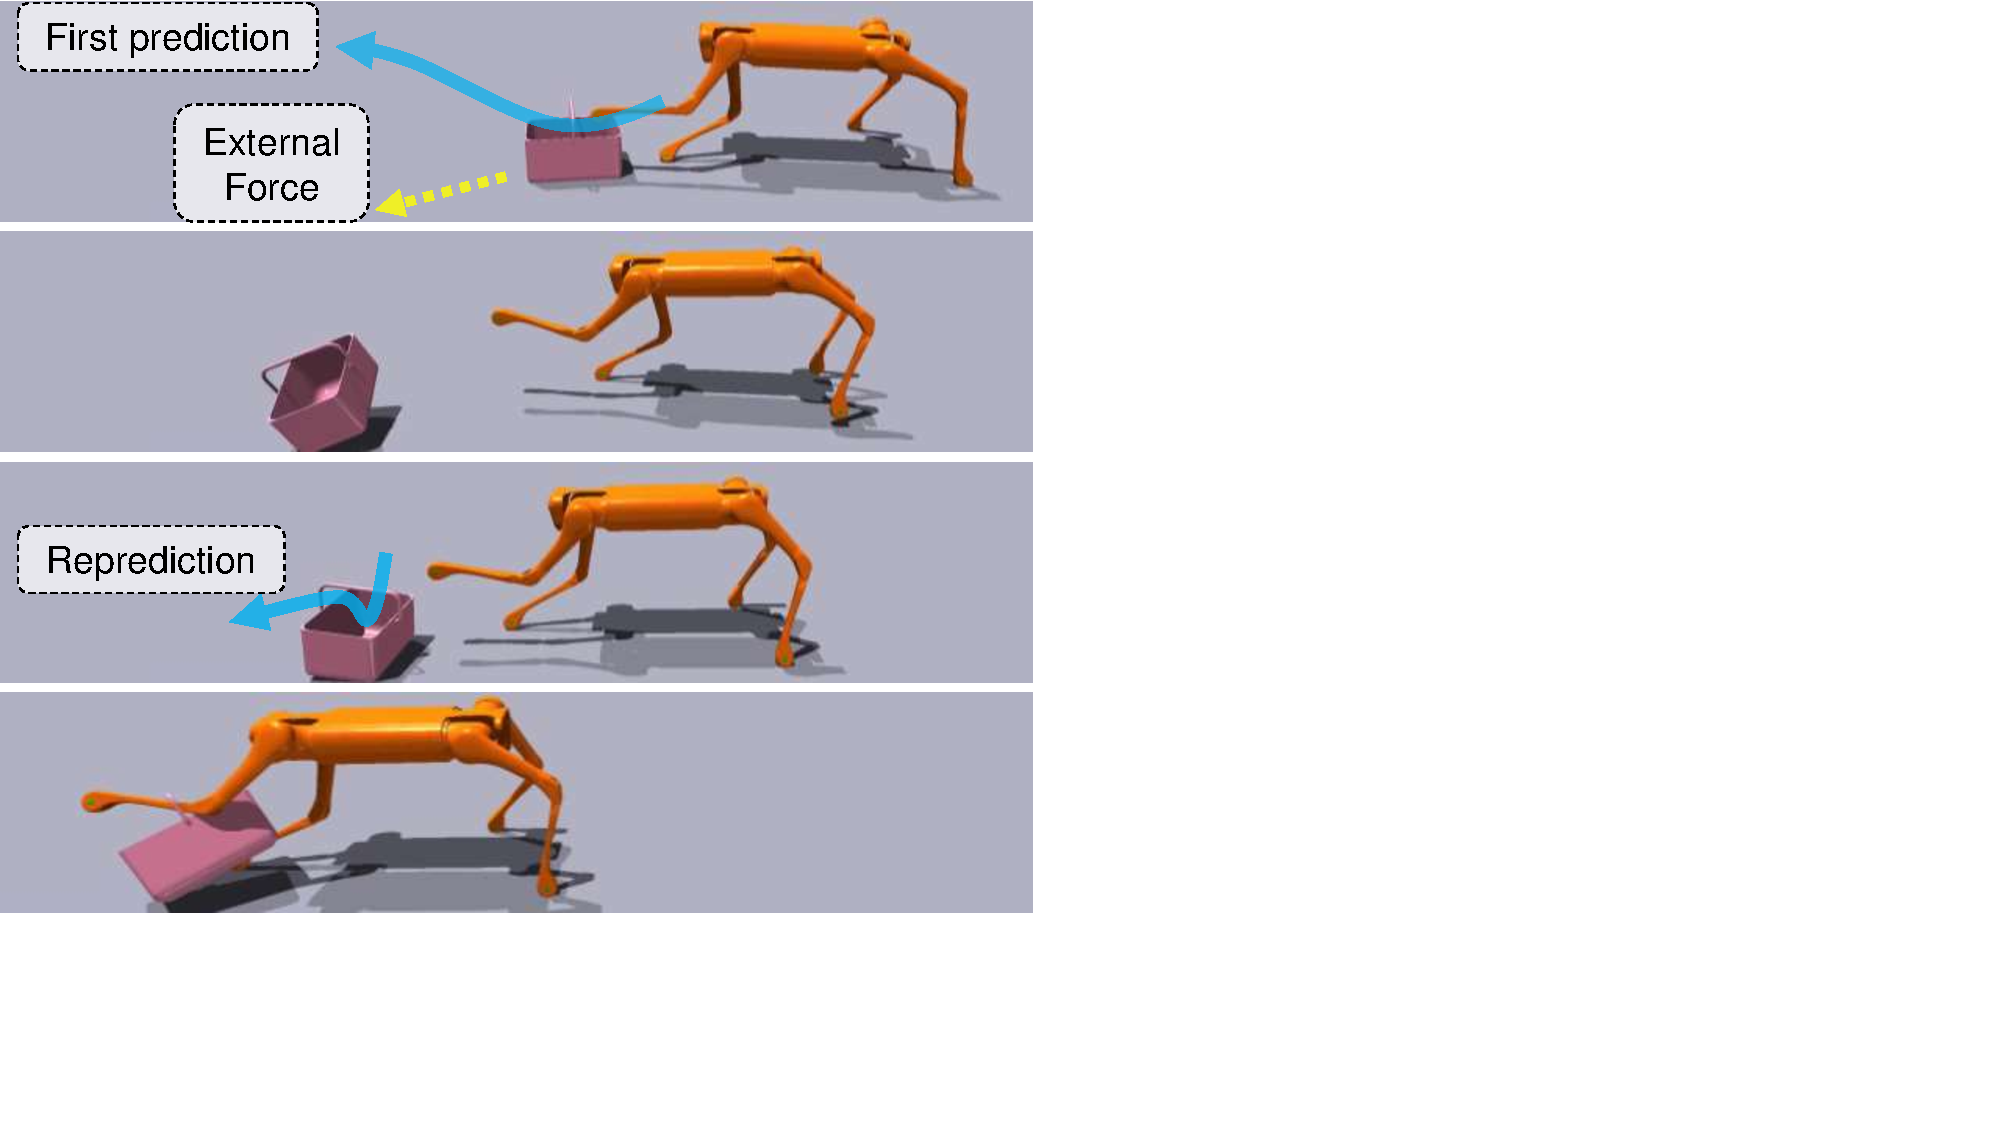
\includegraphics[width=0.99\linewidth, trim={0 35mm 16cm 0}, clip]{figures/decomposed_video/basket_almost_fail.pdf}
%     \caption{\small The performance of our proposed method in the task of lifting a basket when encountering unexpected situations.}
%     \label{fig:planner_basket}
% \end{wrapfigure}
Our expert trajectories are generated in simulation with fixed trajectory parameters, a method that is notably efficient and rapid. However, unlike human video data and teleoperation, this approach does not allow for the collection of data in unexpected situations. Surprisingly, even under these conditions, our method still demonstrated robustness to unforeseen circumstances. 

Taking the task of lifting a basket as an example, we analyze the robot's manipulation process in the face of unexpected events.
As shown in Fig.~\ref{fig:planner_basket}, at the beginning of the episode, the robot predicted the trajectory parameters according to the basket initial pose. During the approach to the basket, we applied random force to the basket, causing it to roll approximately 1.5 meters away. However, the robot quickly repredicted the trajectory parameters based on the new point clouds of the object, allowing the robot to successfully lift the displaced basket.

\begin{figure}[]
    \centering
    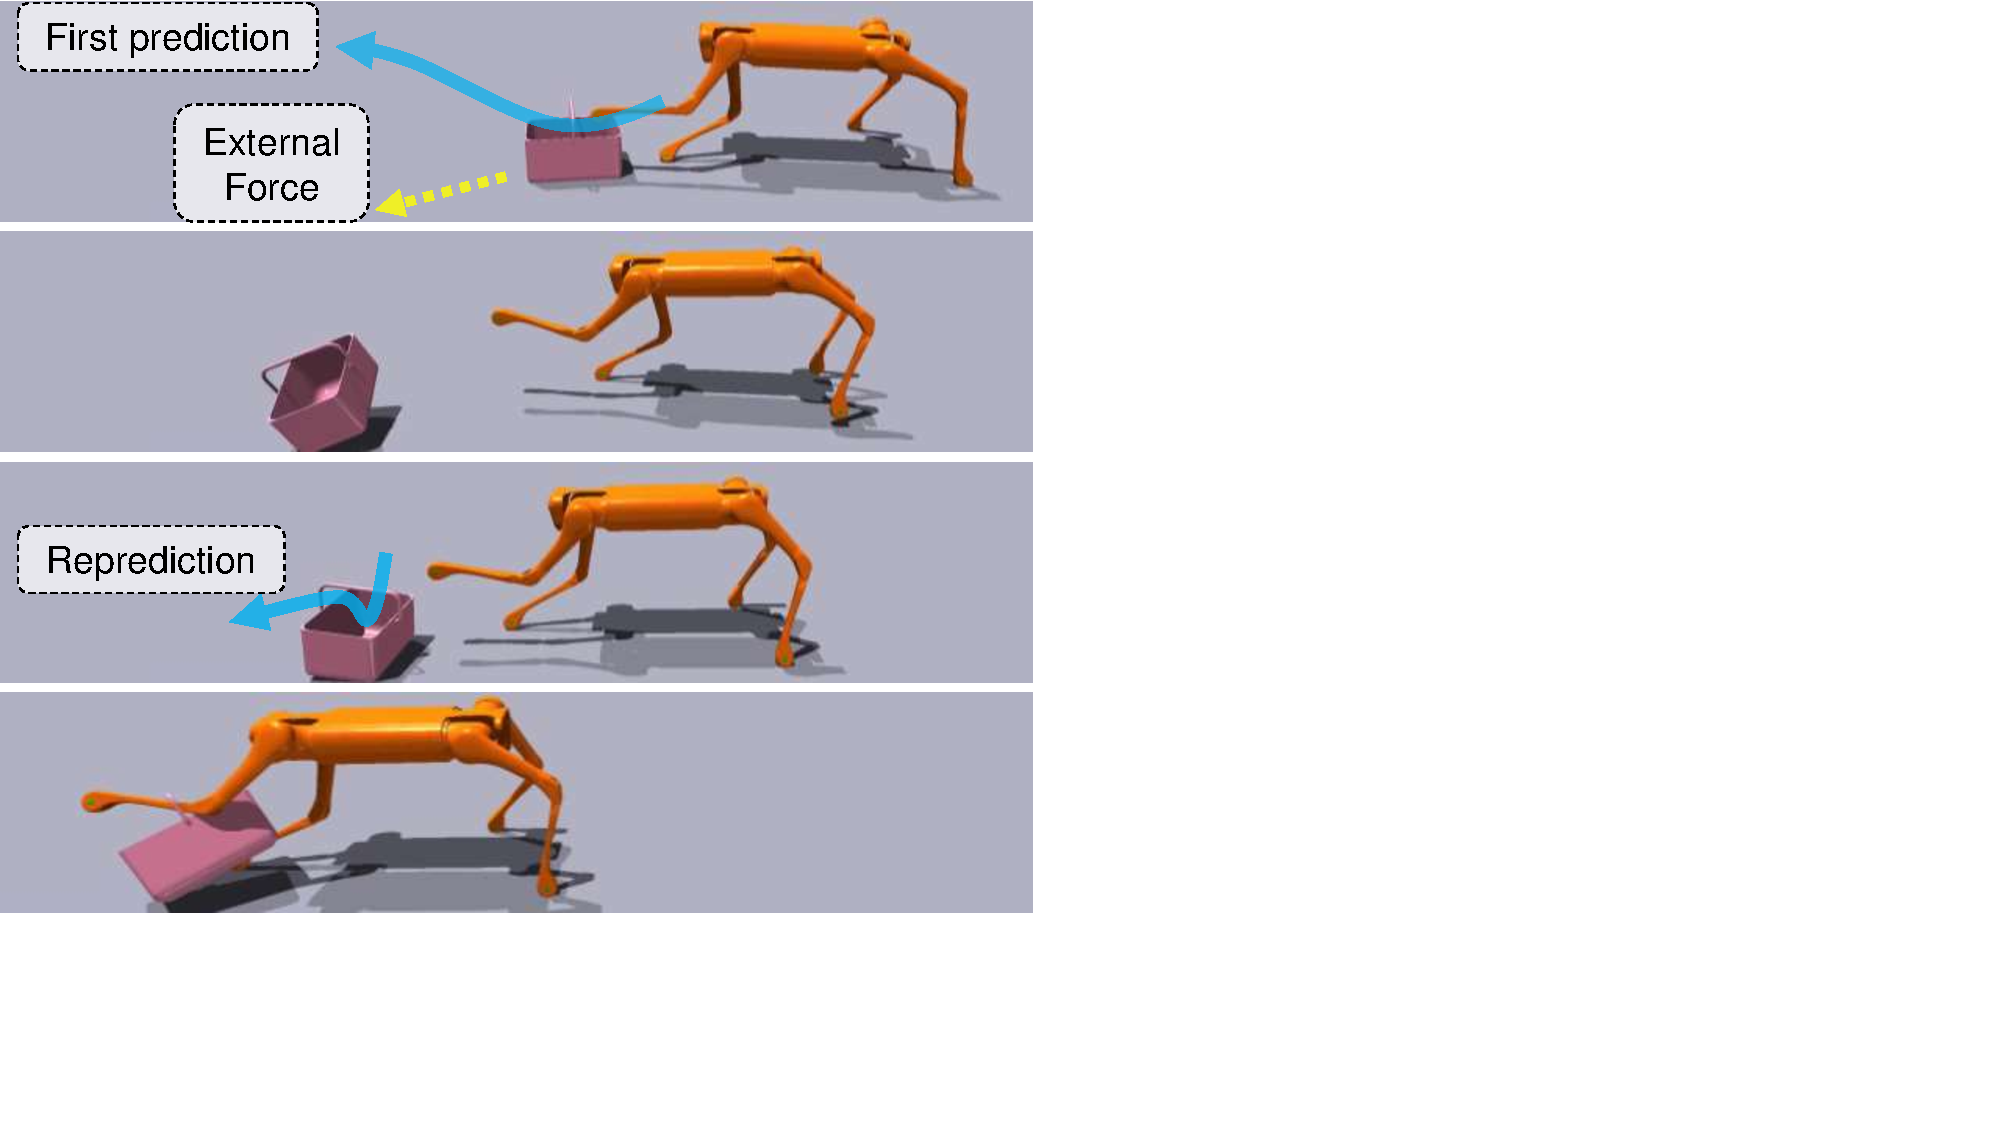
\includegraphics[width=0.99\linewidth, trim={0 35mm 16cm 0}, clip]{figures/decomposed_video/basket_almost_fail.pdf}
    \caption{The performance of our proposed method in the task of lifting a basket when encountering unexpected situations. At the start, the robot estimated the trajectory based on initial pose of basket. When the basket was pushed by external force, the robot quickly updated its trajectory prediction to account for the basket's new pose, enabling it to lift the displaced basket successfully.}
    \label{fig:planner_basket}
    \vspace{-.2in}
\end{figure}


\subsection{Sim2real Transfer}

We directly implement the trained controller and planner on a real-world Aliengo quadruped robot without the need for further fine-tuning, demonstrating the robustness of our approach.
As shown in Fig.~\ref{fig:framework}, the pose of the robot is determined using AprilTag for the coordinate system transformation of trajectory parameters and point clouds. Following this, we applied post-process to the point cloud to ensure alignment with the simulation. In Fig.~\ref{fig:teaser}, we illustrate the robot performing tasks like lifting a basket with its forelimbs and pushing the door during locomotion. For demonstrations of all the skills developed through our method, please refer to the website. 





\subsection{Planner Performance}

\begin{figure}[t]
    \begin{subfigure}[t]{0.470\linewidth}
    \begin{minipage}[t]{\linewidth}
    \centering
    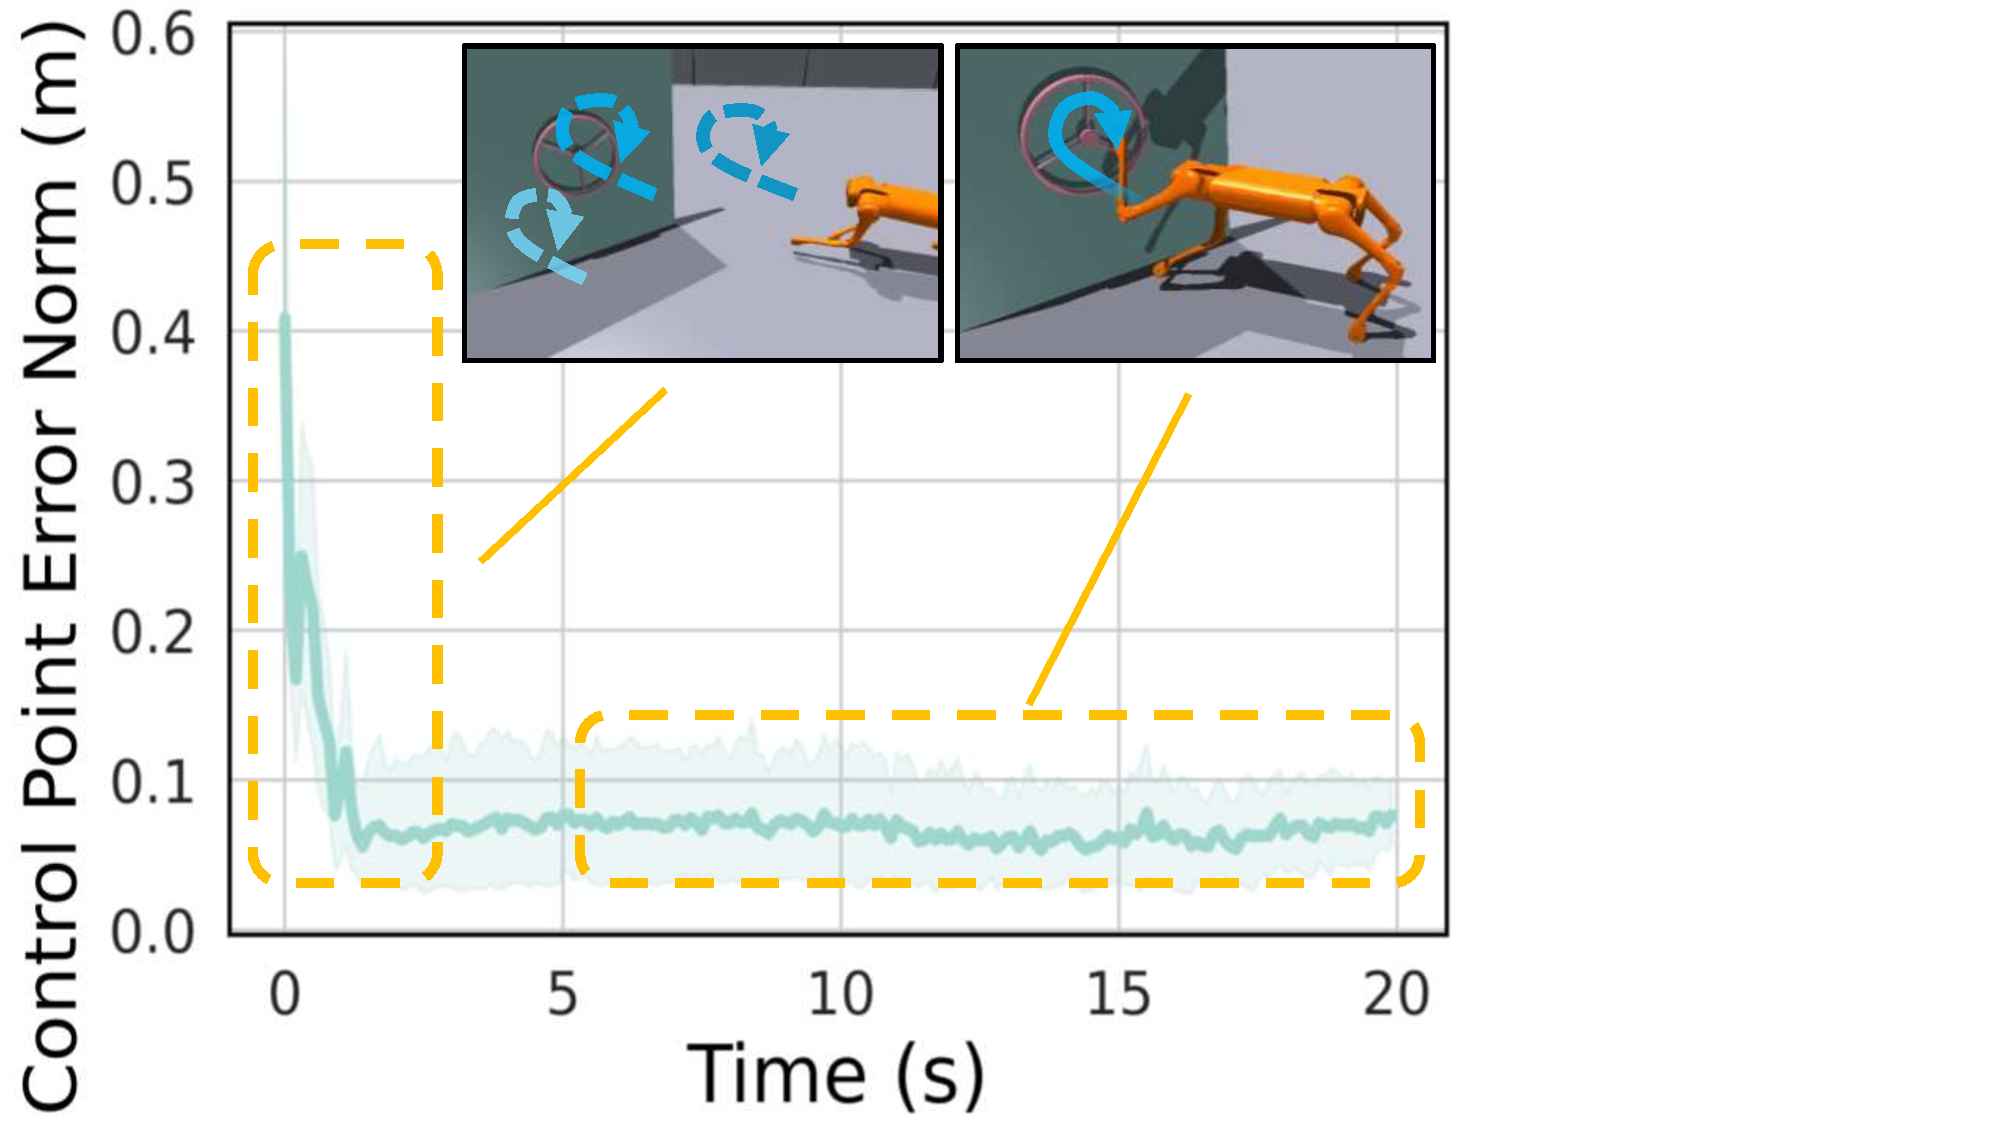
\includegraphics[width=\linewidth, trim={0 0 8cm 0}, clip]{figures/plot/Planner_combined_l.pdf}
    \caption{Valve Twisting Task Performance. The green line displays the differences between the predicted parameters and the expert parameters during the manipulation process, as calculated from data collected during 100 tests.}
    \label{fig:planner_valve}
    \end{minipage}
    \end{subfigure}
    \begin{subfigure}[t]{0.510\linewidth}
    \begin{minipage}[t]{\linewidth}
    \centering
    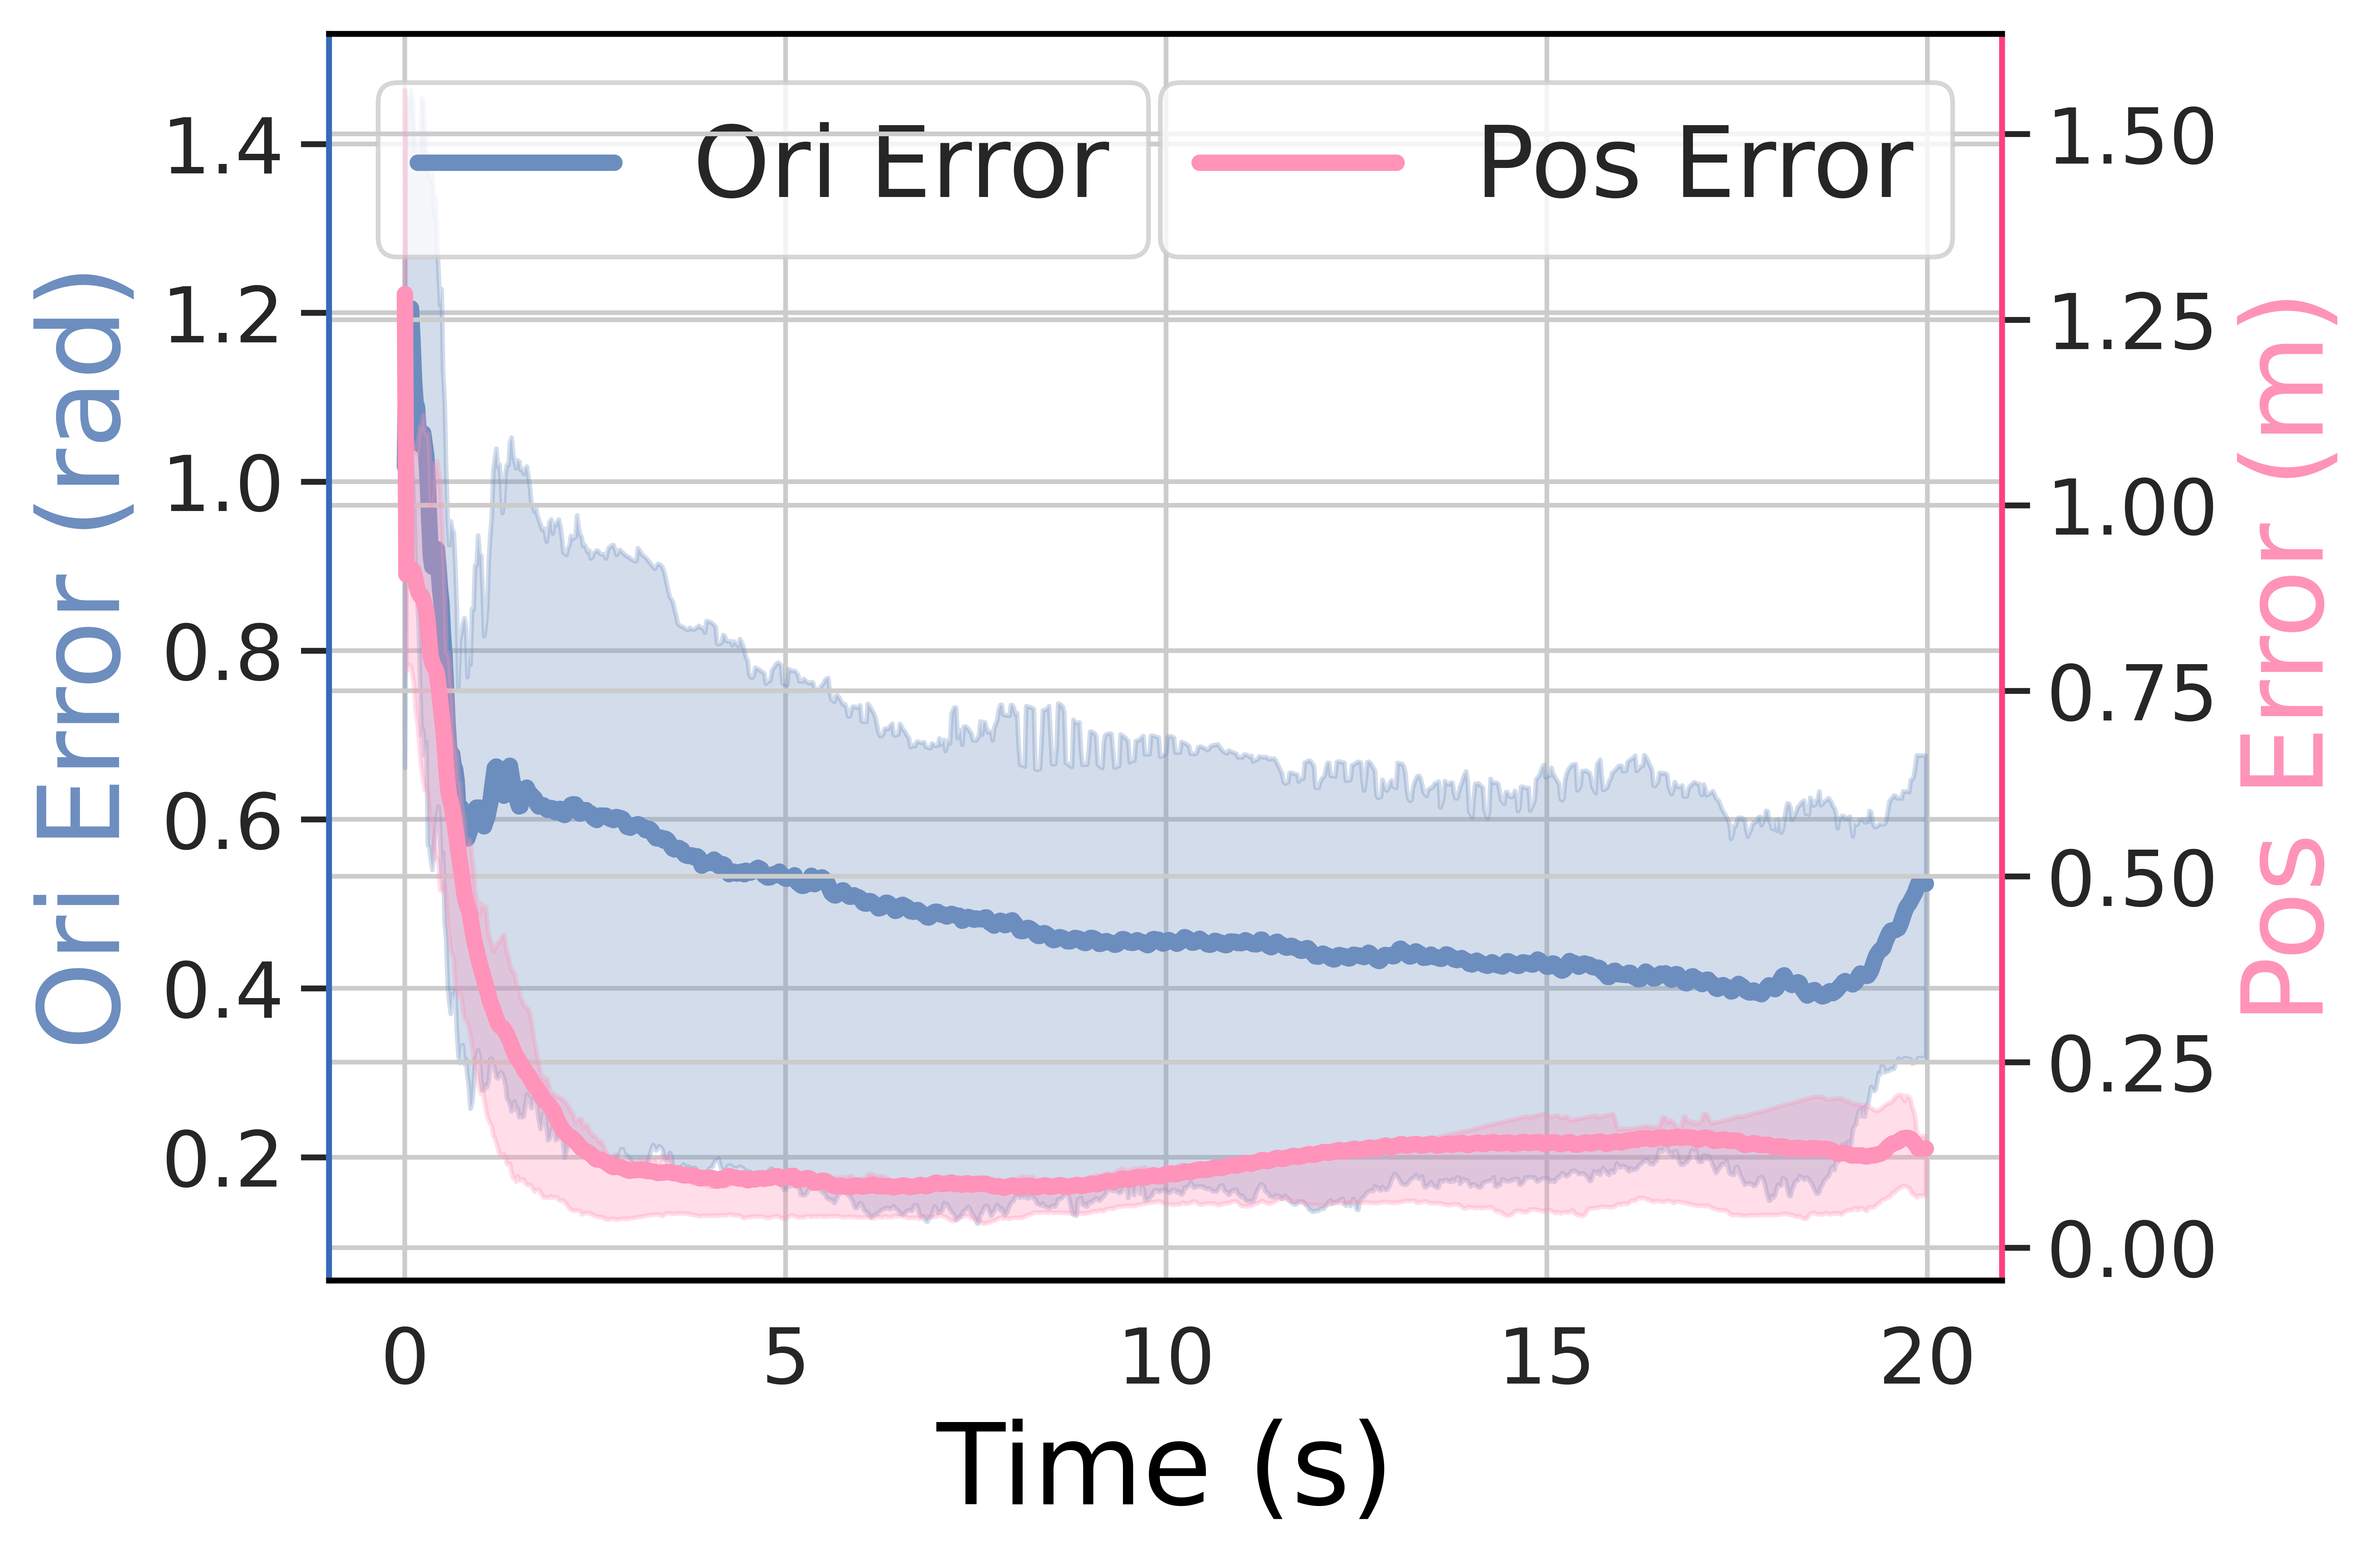
\includegraphics[width=\linewidth]{figures/plot/Controller_Error_l.png}
    \caption{End-effector Trajectory Tracking Performance of the Control Policy. Data on the position and orientation of the end-effector were collected and analyzed during the process of collecting expert demonstrations 10 times for each of the 9 tasks.}
    \label{fig:controller_error}
    \end{minipage}
    \end{subfigure}
    % \hfill
    \captionsetup{justification=raggedright,singlelinecheck=false}
    \caption{The predictive and tracking performance of planners and control policy in simulation.}
    \vspace{-.2in}
\end{figure}


The trained planner is capable of predicting the trajectory parameters based on the point clouds and transmitting them to the controller, enabling the robot to complete challenging loco-manipulation tasks, as shown in Fig.~\ref{fig:tasks}.

We conduct an in-depth test of the planner's performance, using the valve twisting task as an example for analysis.
As shown in Fig.~\ref{fig:planner_valve}, at the beginning of the episode, the predicted parameters are constantly changing, leading to a rather chaotic predicted trajectory. As the manipulation progresses, the predicted trajectory tends to converge.




\subsection{Control Policy Performance}

\textbf{Robust tracking against disturbances.}
We test the tracking performance of the control policy. In the tests, the robot is required to follow the expert trajectories for 9 different tasks and record the position and orientation errors of the end-effector in comparison to the desired value. 

As shown in Fig.~\ref{fig:controller_error}, both position and orientation errors peaked when the manipulation began, then position error converged to the lowest value after approximately 3 seconds. In the latter half of the episode, due to the contact with objects, position errors slightly increased but still remained at a low level.
Note that precise tracking of both the position and orientation of the EE is typically unsolvable, given the system is highly underactuated. Our system opts to prioritize position tracking, resulting in the reduction of the minimum orientation error to 0.4 radians. %This level of accuracy is sufficient for completing most tasks.



\textbf{Teleoperation with control policy.}
\begin{figure}[]
    \centering
    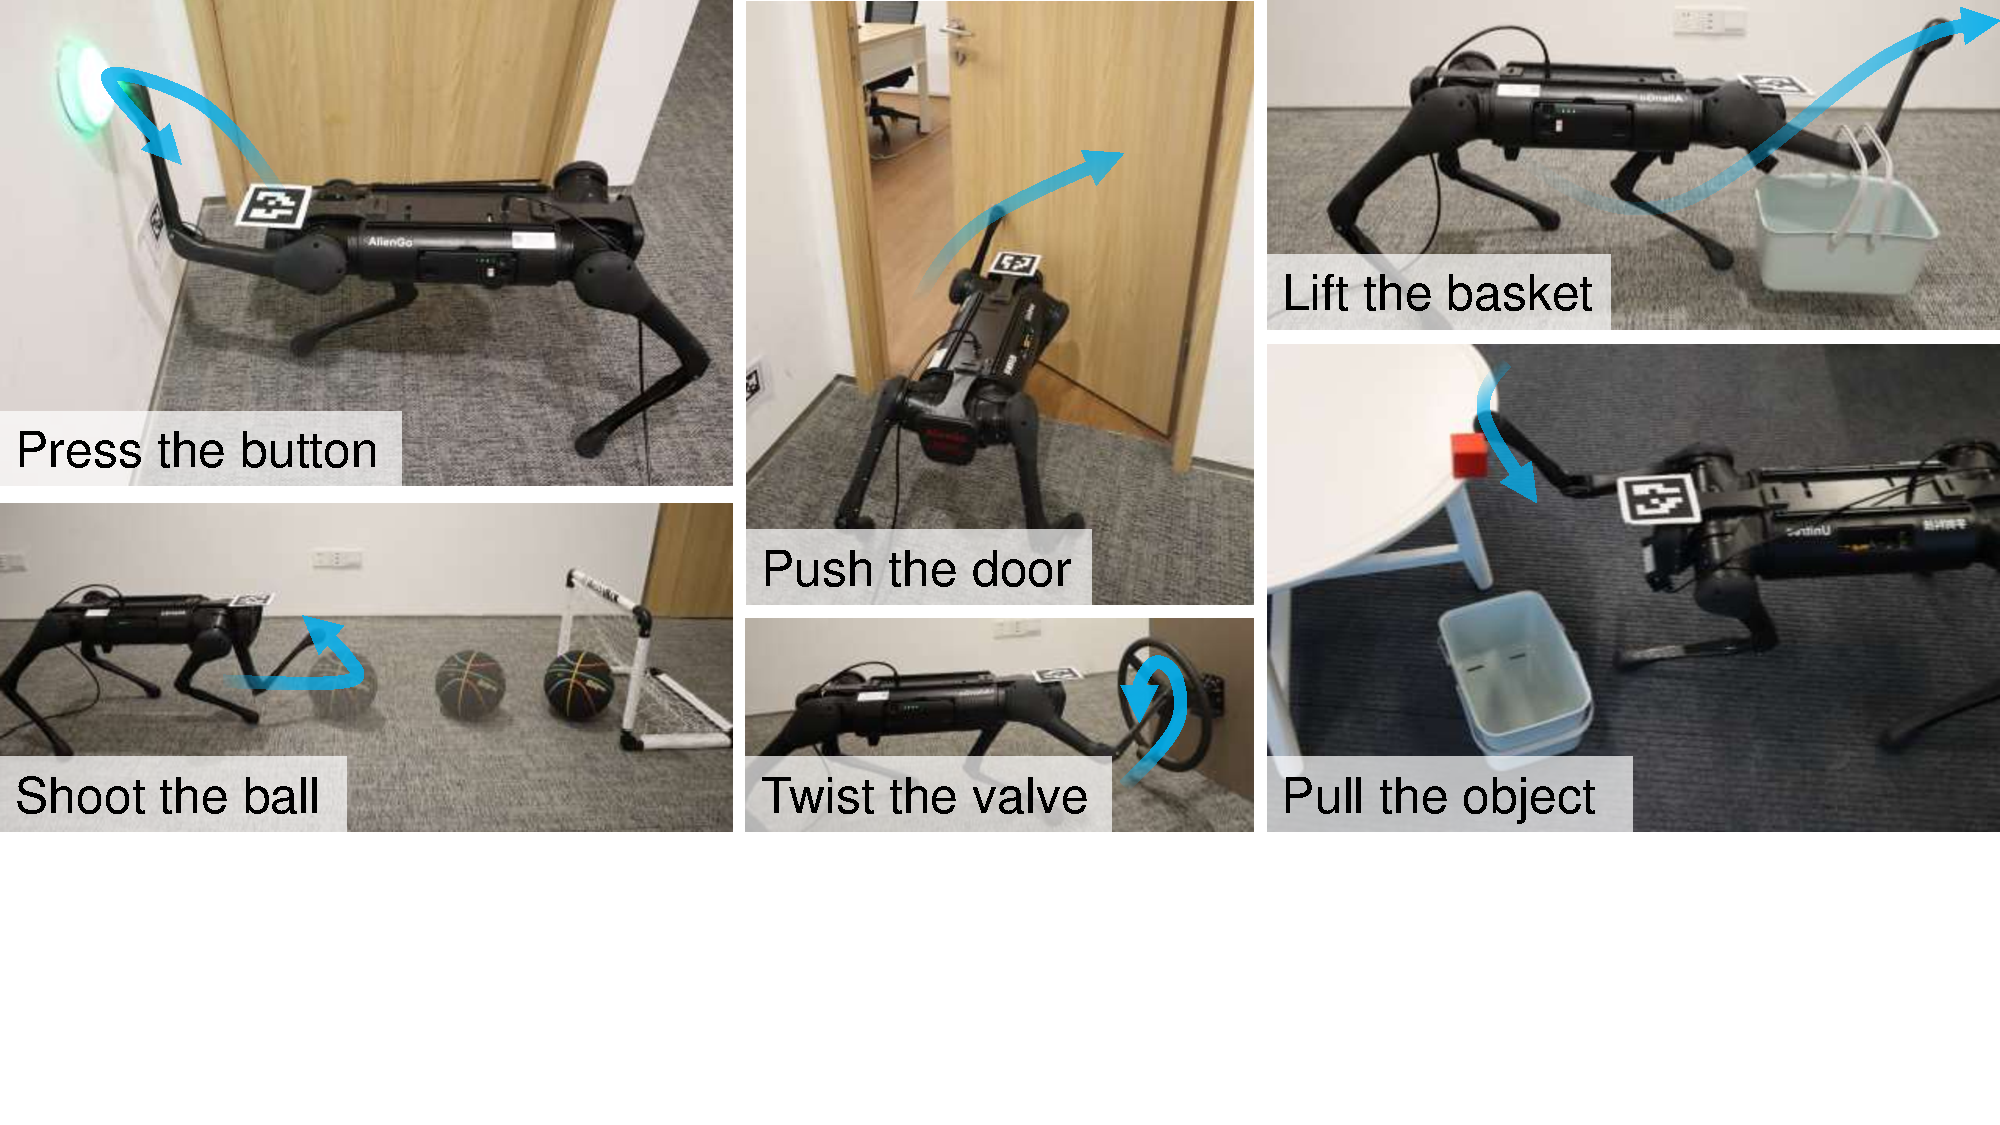
\includegraphics[width=0.495\textwidth, trim={0 5cm 0 0}, clip]{figures/tasks/teleop.pdf}
    \caption{Teleoperation in real world with control policy. We accomplish the above tasks in the real world by the low-level controller with specific trajectory parameters via a joystick.}
    \label{fig:teleop}
    \vspace{-.2in}
\end{figure}
Besides autonomous manipulation, we can \emph{also} collect data via teleopration. As shown in Fig.~\ref{fig:teleop}, using the trained low-level controller, we executed a series of real-world experiments on the robot, guided by specific trajectory parameters. These experiments show that our low-level controller can effectively perform a variety of daily tasks in real-world settings, tasks that previously necessitated a robotic arm. 
